\documentclass[10pt,letterpaper]{article}
\usepackage[margin=0.62in,headheight=20pt,footskip=24pt]{geometry}
\usepackage[scaled=0.95]{helvet}
\renewcommand{\familydefault}{\sfdefault}
\usepackage{amsmath,amssymb,array,booktabs,enumitem,graphicx,tabularx,xcolor}
\usepackage[colorlinks=true,linkcolor=TEJBlue,urlcolor=TEJBlue]{hyperref}
\usepackage{fancyhdr,lastpage}

\definecolor{TEJNavy}{HTML}{1E2B55}
\definecolor{TEJBlue}{HTML}{1769AA}
\definecolor{TEJOrange}{HTML}{E97828}
\definecolor{TEJPale}{HTML}{F3F6FA}
\definecolor{TEJRule}{HTML}{B8C2D1}
\definecolor{TEJGreen}{HTML}{2C7A4B}

\pagestyle{fancy}
\fancyhf{}
\lhead{\color{TEJNavy}\small TEJ Electronics}
\rhead{\color{TEJNavy}\small Two Loops to a Matrix}
\cfoot{\color{TEJNavy}\small Page \thepage\ of \pageref{LastPage}}
\renewcommand{\headrulewidth}{0.4pt}
\renewcommand{\headrule}{\hbox to\headwidth{\color{TEJRule}\leaders\hrule height \headrulewidth\hfill}}

\setlength{\parindent}{0pt}
\setlength{\parskip}{5pt}
\setlist[itemize]{leftmargin=1.3em,itemsep=2pt,topsep=3pt}
\setlist[enumerate]{leftmargin=1.55em,itemsep=3pt,topsep=3pt}
\renewcommand{\arraystretch}{1.25}

\newcommand{\sectiontitle}[1]{%
  {\color{TEJOrange}\Large\bfseries #1}\par
  {\color{TEJRule}\rule{\linewidth}{1.1pt}}\vspace{4pt}
}
\newcommand{\steptitle}[2]{%
  \noindent\colorbox{TEJBlue}{\parbox{0.075\linewidth}{\centering\color{white}\Large\bfseries #1}}%
  \hspace{0.012\linewidth}%
  \colorbox{TEJPale}{\parbox{0.875\linewidth}{\color{TEJNavy}\large\bfseries #2}}\par\vspace{5pt}
}
\newcommand{\keybox}[1]{%
  \begin{center}
  \fcolorbox{TEJOrange}{TEJPale}{\parbox{0.91\linewidth}{#1}}
  \end{center}
}
\newcommand{\writebox}[1]{%
  \par\vspace{8pt}{\color{TEJRule}\noindent\rule{\linewidth}{0.5pt}\par\vspace{0.24in}%
  \noindent\rule{\linewidth}{0.5pt}\par\vspace{0.24in}%
  \noindent\rule{\linewidth}{0.5pt}}\par\vspace{4pt}
}
\newcommand{\kiloohm}{\mathrm{k}\Omega}

\begin{document}
\color{TEJNavy}

% ---------------------------------------------------------------------------
% Page 1
% ---------------------------------------------------------------------------
\begin{center}
  {\color{TEJOrange}\rule{\linewidth}{3pt}}\\[13pt]
  {\fontsize{28}{32}\selectfont\bfseries From Two Loops to a Matrix}\\[7pt]
  {\Large A guided Kirchhoff and Jupyter bridge}\\[10pt]
  {\color{TEJOrange}\rule{0.72\linewidth}{2pt}}
\end{center}

\vspace{8pt}
\begin{tabularx}{\linewidth}{@{}>{\bfseries}l X@{}}
Student number and last name: & \hrulefill \\[8pt]
Class or period: & \hrulefill \\
\end{tabularx}

\sectiontitle{Learning goals}

By the end of this bridge, I can:
\begin{itemize}
  \item define the three current directions in a two-loop circuit;
  \item write one KVL equation for each loop and handle the shared resistor;
  \item rearrange both equations into the same variable order;
  \item build $A\mathbf{x}=\mathbf{b}$ and solve it numerically and symbolically;
  \item verify the result with KCL, KVL, and a residual.
\end{itemize}

\sectiontitle{Why this is useful}

Two loops share one component, so the current through that component depends on both loop currents. A matrix does not replace Kirchhoff's laws. It organizes the equations after the circuit reasoning is complete.

\sectiontitle{What you will make}

You will submit one notebook showing this complete chain:

\[
\boxed{\text{arrows}}\;\longrightarrow\;
\boxed{\text{two KVL equations}}\;\longrightarrow\;
\boxed{\text{standard form}}\;\longrightarrow\;
\boxed{A\mathbf{x}=\mathbf{b}}\;\longrightarrow\;
\boxed{\text{two solver methods}}\;\longrightarrow\;
\boxed{\text{checks}}
\]

\sectiontitle{Before you start}

\begin{itemize}
  \item Use Question 4 as the worked model, then transfer the method to Question 5.
  \item Keep the released Question 5 answer closed until your matrix rows read back correctly.
  \item Download the course notebook from the assignment page.
  \item Keep resistance in $\kiloohm$, voltage in V, and current in mA.
  \item This checkpoint is a computational verification activity. No physical lab is required.
\end{itemize}

\textbf{Textbook support:} \href{https://drive.google.com/file/d/1RXDje9v9TuuNF4V1Jlqemcsn1qJlKcjz/view}{Grob, Chapter 9, pp. 264--281}.
\textbf{Practice support:} \href{https://drive.google.com/file/d/125X4YkWq2HO8evqYM9jRUuKPsbMXHhdG/view}{Problems Manual, Chapter 9}.\\
\textbf{Engagement review:} \href{https://www.youtube.com/watch?v=d-a9Pr2z-qg}{ElectroBOOM101-008: Kirchhoff Circuit Laws}.

\newpage

% ---------------------------------------------------------------------------
% Page 2
% ---------------------------------------------------------------------------
\sectiontitle{Start with current directions and the shared branch}

\steptitle{1}{Define the variables before writing equations}

For the completed Question 4 circuit, use clockwise mesh currents $I_1$ and $I_2$. The two mesh currents move through the shared resistor in opposite directions. Define $I_3$ downward through the shared resistor.

\keybox{%
\centering
\Large
$I_1-I_2-I_3=0\quad\Longrightarrow\quad I_3=I_1-I_2$
\par\smallskip
\normalsize This is KCL at the shared branch. It fixes the meaning of every later sign.
}

\begin{center}
\begin{tabular}{>{\bfseries}c p{0.67\linewidth}}
$I_1$ & clockwise current assigned to Loop 1 \\
$I_2$ & clockwise current assigned to Loop 2 \\
$I_3$ & downward current through $R_3$, defined as $I_1-I_2$ \\
\end{tabular}
\end{center}

\steptitle{2}{Use one sign rule from start to finish}

As you walk around a loop:

\begin{center}
\begin{tabularx}{0.9\linewidth}{@{}>{\bfseries}l X@{}}
Source from $-$ to $+$ & voltage rise: write $+V_S$ \\
Source from $+$ to $-$ & voltage drop: write $-V_S$ \\
Resistor in the current direction & voltage drop: write $-IR$ \\
Resistor against the current direction & voltage rise: write $+IR$ \\
\end{tabularx}
\end{center}

\keybox{%
\textbf{Essential skill:} do not jump directly to the matrix. First write the signed KVL terms in the order encountered around each loop. Then substitute $I_3=I_1-I_2$.
}

\textbf{Quick check before continuing}

If the final value of $I_3$ is negative, what would that mean?\\
\writebox{0.72in}

\newpage

% ---------------------------------------------------------------------------
% Page 3
% ---------------------------------------------------------------------------
\sectiontitle{Loop 1: write, substitute, expand, and collect}

\steptitle{3}{Walk clockwise around Loop 1}

\begin{center}
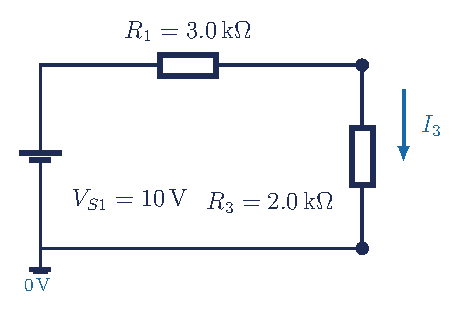
\includegraphics[width=0.70\linewidth]{../schematics/kirchhoff-q4-loop1-clean.pdf}
\end{center}

\begin{center}
\begin{tabular}{c c c}
\toprule
Element & Signed KVL term & Reason \\
\midrule
$V_{S1}=10\,\mathrm{V}$ & $+10$ & rise through the source \\
$R_1=3.0\,\kiloohm$ & $-3I_1$ & travel with $I_1$ \\
$R_3=2.0\,\kiloohm$ & $-2I_3$ & travel with the defined $I_3$ \\
\bottomrule
\end{tabular}
\end{center}

\textbf{Write the voltage changes before substituting Ohm's law:}
\[
+10-V_{R1}-V_{R3}=0
\]

\textbf{Replace each resistor voltage with $IR$:}
\[
V_{R1}=I_1R_1=3I_1,\qquad V_{R3}=I_3R_3=2I_3
\]
\[
+10-3I_1-2I_3=0
\]

\textbf{Substitute the shared current:}
\[
+10-3I_1-2(I_1-I_2)=0
\]

\textbf{Distribute $-2$ to both terms in the bracket:}
\[
+10-3I_1-2I_1+2I_2=0
\]

\textbf{Collect the two $I_1$ terms:}
\[
+10-5I_1+2I_2=0
\]

\textbf{Subtract 10 from both sides, then multiply every term by $-1$:}
\[
-5I_1+2I_2=-10
\quad\Longrightarrow\quad
\boxed{5I_1-2I_2=10}
\]

\keybox{%
The first matrix row is read directly from the standard-form equation: coefficient of $I_1$, coefficient of $I_2$, right side. Therefore Row 1 is $[5,\,-2]$ and $b_1=10$.
}

\newpage

% ---------------------------------------------------------------------------
% Page 4
% ---------------------------------------------------------------------------
\sectiontitle{Loop 2: the shared resistor changes sign}

\steptitle{4}{Walk clockwise around Loop 2}

\begin{center}
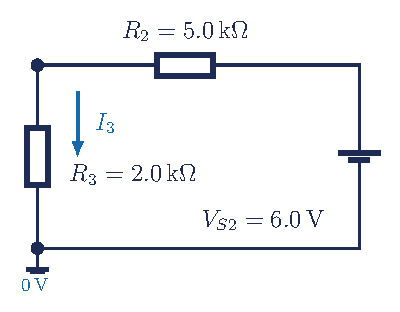
\includegraphics[width=0.70\linewidth]{../schematics/kirchhoff-q4-loop2-clean.pdf}
\end{center}

\begin{center}
\begin{tabular}{c c c}
\toprule
Element & Signed KVL term & Reason \\
\midrule
$V_{S2}=6.0\,\mathrm{V}$ & $+6$ & rise through the source \\
$R_2=5.0\,\kiloohm$ & $-5I_2$ & travel with $I_2$ \\
$R_3=2.0\,\kiloohm$ & $+2I_3$ & travel against the defined $I_3$ \\
\bottomrule
\end{tabular}
\end{center}

\textbf{Write the voltage changes before substituting Ohm's law:}
\[
+6-V_{R2}+V_{R3}=0
\]

\textbf{Replace each resistor voltage with $IR$:}
\[
V_{R2}=I_2R_2=5I_2,\qquad V_{R3}=I_3R_3=2I_3
\]
\[
+6-5I_2+2I_3=0
\]

\textbf{Substitute the shared current:}
\[
+6-5I_2+2(I_1-I_2)=0
\]

\textbf{Distribute $+2$ to both terms in the bracket:}
\[
+6-5I_2+2I_1-2I_2=0
\]

\textbf{Reorder the current terms, then combine the $I_2$ terms:}
\[
+6+2I_1-5I_2-2I_2=0
\quad\Longrightarrow\quad
+6+2I_1-7I_2=0
\]

\textbf{Subtract 6 from both sides:}
\[
2I_1-7I_2=-6
\]

\textbf{Multiply the complete equation by $-1$:}
\[
\boxed{-2I_1+7I_2=6}
\]

\keybox{%
The second matrix row is $[-2,\,7]$ and $b_2=6$. Multiplying a complete equation by $-1$ does not change its solution.
}

% ---------------------------------------------------------------------------
% Page 5 continues after the detailed Loop 2 derivation
% ---------------------------------------------------------------------------
\sectiontitle{Put both equations into one matrix}

\steptitle{5}{Align the variable order}

Use the same order, $[I_1,I_2]$, in every equation and every matrix row.

\begin{align*}
\text{Equation 1:}\qquad & 5I_1-2I_2=10 \\
\text{Equation 2:}\qquad & -2I_1+7I_2=6
\end{align*}

\begin{center}
\begin{tabular}{c c c c}
\toprule
 & coefficient of $I_1$ & coefficient of $I_2$ & right side \\
\midrule
Equation 1 & $5$ & $-2$ & $10$ \\
Equation 2 & $-2$ & $7$ & $6$ \\
\bottomrule
\end{tabular}
\end{center}

\[
\underbrace{\begin{bmatrix}
5 & -2\\
-2 & 7
\end{bmatrix}}_{A\;[\kiloohm]}
\underbrace{\begin{bmatrix}
I_1\\I_2
\end{bmatrix}}_{\mathbf{x}\;[\mathrm{mA}]}
=
\underbrace{\begin{bmatrix}
10\\6
\end{bmatrix}}_{\mathbf{b}\;[\mathrm{V}]}
\]

\textbf{Expand the matrix product row by row:}
\[
\begin{bmatrix}
5I_1+(-2)I_2\\
(-2)I_1+7I_2
\end{bmatrix}
=
\begin{bmatrix}10\\6\end{bmatrix}
\]

The top row is Equation 1. The bottom row is Equation 2. If either row reads back differently from the KVL equation, fix the matrix before solving.

\keybox{%
\centering
$[\kiloohm][\mathrm{mA}]=[\mathrm{V}]$\\[3pt]
The unit choice makes the numerical answer come out in milliamperes.
}

\steptitle{6}{Use the row rule to catch transcription errors}

For each row, read the matrix back as an equation before solving:

\[
[5,\,-2]\begin{bmatrix}I_1\\I_2\end{bmatrix}=10
\quad\Longrightarrow\quad 5I_1-2I_2=10
\]

\[
[-2,\,7]\begin{bmatrix}I_1\\I_2\end{bmatrix}=6
\quad\Longrightarrow\quad -2I_1+7I_2=6
\]

\textbf{Stumbling block:} changing the variable order in only one row creates a different problem. The solver may still return a clean-looking answer.

\newpage

% ---------------------------------------------------------------------------
% Page 6
% ---------------------------------------------------------------------------
\sectiontitle{Solve two ways and verify}

\steptitle{7}{Numerical linear algebra}

Use a solver for $A\mathbf{x}=\mathbf{b}$. Do not calculate $A^{-1}$ by hand for this task.

\begin{verbatim}
import numpy as np

A = np.array([[5.0, -2.0],
              [-2.0, 7.0]])
b = np.array([10.0, 6.0])
x = np.linalg.solve(A, b)
residual = A @ x - b
\end{verbatim}

\steptitle{8}{Symbolic solution}

Symbolic algebra keeps exact fractions instead of decimal approximations.

\begin{verbatim}
import sympy as sp

I1, I2 = sp.symbols("I1 I2")
equations = [sp.Eq(5*I1 - 2*I2, 10),
             sp.Eq(-2*I1 + 7*I2, 6)]
exact = sp.solve(equations, (I1, I2), dict=True)[0]
\end{verbatim}

The exact solution is

\[
I_1=\frac{82}{31}\,\mathrm{mA},
\qquad
I_2=\frac{50}{31}\,\mathrm{mA},
\qquad
I_3=I_1-I_2=\frac{32}{31}\,\mathrm{mA}.
\]

\steptitle{9}{Verify independently}

\begin{align*}
\text{Equation 1:}\quad 5\left(\frac{82}{31}\right)-2\left(\frac{50}{31}\right)&=10 \\
\text{Equation 2:}\quad -2\left(\frac{82}{31}\right)+7\left(\frac{50}{31}\right)&=6 \\
\text{KCL:}\quad \frac{82}{31}-\frac{50}{31}&=\frac{32}{31}
\end{align*}

\keybox{%
A near-zero residual proves that the calculated currents satisfy the equations entered into Python. It does not prove that the arrows, signs, units, or original circuit model were correct.
}

\newpage

% ---------------------------------------------------------------------------
% Page 7
% ---------------------------------------------------------------------------
\sectiontitle{Part B: build the Question 5 matrix yourself}

\textbf{The goal:} use the same method on Question 5 without being given its coefficients, completed matrix, or currents.

\steptitle{10}{Define the currents and signs}

In the notebook, answer before doing algebra:
\begin{enumerate}
  \item What directions did you choose for $I_1$, $I_2$, and $I_3$?
  \item Is your shared-current equation $I_3=I_1-I_2$ or $I_3=I_2-I_1$? Why?
  \item Which source and resistor terms are rises? Which are drops?
  \item Why does the shared-resistor sign differ between the two loop walks?
\end{enumerate}

\steptitle{11}{Show seven algebra lines for each loop}

For \textbf{each} loop, show one move per line:
\begin{enumerate}
  \item signed KVL using resistor-voltage symbols;
  \item replace every resistor voltage with $IR$;
  \item substitute the expression for $I_3$;
  \item distribute through the bracket;
  \item reorder into $[I_1,I_2]$;
  \item combine like terms;
  \item move the constant to the right side.
\end{enumerate}

Your two boxed equations should have the structure
\[
\boxed{a_{11}I_1+a_{12}I_2=b_1},
\qquad
\boxed{a_{21}I_1+a_{22}I_2=b_2}.
\]

\steptitle{12}{Extract coefficients and prove the matrix matches}

\begin{center}
\begin{tabular}{c c c c}
\toprule
Question 5 & coefficient of $I_1$ & coefficient of $I_2$ & right side \\
\midrule
Equation 1 & \rule{0.75in}{0.4pt} & \rule{0.75in}{0.4pt} & \rule{0.75in}{0.4pt} \\
Equation 2 & \rule{0.75in}{0.4pt} & \rule{0.75in}{0.4pt} & \rule{0.75in}{0.4pt} \\
\bottomrule
\end{tabular}
\end{center}

\[
\underbrace{\begin{bmatrix}a_{11}&a_{12}\\a_{21}&a_{22}\end{bmatrix}}_{A}
\underbrace{\begin{bmatrix}I_1\\I_2\end{bmatrix}}_{\mathbf{x}}
=
\underbrace{\begin{bmatrix}b_1\\b_2\end{bmatrix}}_{\mathbf{b}}
\]

Replace the six placeholders with your numbers. Read the top row back as Equation 1 and the bottom row as Equation 2. Only then use Jupyter to solve and compare with the released answer.

\keybox{%
The helper questions reveal the method, not the answer. Your algebra must generate the six numbers placed into $A$ and $\mathbf{b}$.
}

\newpage

% ---------------------------------------------------------------------------
% Page 8
% ---------------------------------------------------------------------------
\sectiontitle{Assignment and submission}

\textbf{Part A:} explain how the completed Question 4 circuit becomes two equations, one matrix, and two matching solver results.

\textbf{Part B:} use the helper questions to derive the Question 5 equations and matrix without copying the completed answer.

\textbf{The essential skill:} keep the shared-current definition and variable order consistent.

\textbf{The challenge:} explain every sign in both loop equations instead of copying the finished matrix.

\textbf{The investigation:} use Python help and the official NumPy or SymPy documentation when a function or object is unfamiliar.

\textbf{The verification:} use residuals, substitution, and $I_3=I_1-I_2$.

\textbf{The reflection:} identify the step that changed your understanding of the two loops.

\subsection*{Required notebook evidence}

\begin{enumerate}
  \item Write the definitions of $I_1$, $I_2$, and $I_3$ in a Markdown cell.
  \item Show the three signed KVL terms for Loop 1 and derive Equation 1.
  \item Show the three signed KVL terms for Loop 2 and derive Equation 2.
  \item State the variable order and units.
  \item Build $A$ and $\mathbf{b}$, then read both matrix rows back as equations.
  \item Solve with `numpy.linalg.solve` and report the residual vector.
  \item Solve the same equations with `sympy.solve` and report exact fractions.
  \item Calculate $I_3$ and compare all three currents with the released answer.
  \item Answer the notebook reflection in complete sentences.
  \item For Question 5, show both seven-line rearrangements, the coefficient table, the completed matrix, and both row read-backs.
  \item Solve Question 5 only after the matrix is justified; then compare with the released answer.
\end{enumerate}

\subsection*{Progressive hints}

\textbf{Hint 1 - concept:} the shared resistor carries $I_1-I_2$ because the mesh currents oppose each other there.\\
\textbf{Hint 2 - documentation:} search `numpy.linalg.solve A shape` or `SymPy solve simultaneous equations`.\\
\textbf{Hint 3 - technical:} use rows $[5,-2]$ and $[-2,7]$ only after you can read them back as the two standard-form equations.

\subsection*{Submit}

Rename the notebook exactly:

\begin{center}
\texttt{studentnumber-lastname-kirchhoff-jupyter.ipynb}
\end{center}

Example: \texttt{123456789-Smith-kirchhoff-jupyter.ipynb}. Keep the `.ipynb` ending. Restart the kernel, run all required cells, save, download, reopen, and submit the notebook through the assigned classroom system.

\textbf{Later, not tomorrow:} the intentional keyword error, array-shape error, unit bug, parameter sweep, capacitors, and RC response.

\end{document}
